\chapter{Introduzione}
\addcontentsline{toc}{chapter}{Introduzione}
La realizzazione di un sistema digitale complesso è possibile mediante due diverse strategie realizzative basilari: la sintesi in \textit{hardware diretto} e la sintesi in \textit{logica programmata}.
Entrambe queste metodologie realizzative, seppur presentando differenze architetturali sostanziali, possono garantire la sintesi di due sistemi digitali assolutamente equivalenti dal punto di vista del legame ingresso-uscita, che mantengano ossia prestazioni funzionali invariate. \newline
La scelta della metodologia di realizzazione di un sistema digitale dipende dalle circostanze strettamente legate alla funzionalità del sistema da realizzare. Ogni soluzione presenta i propri vantaggi e svantaggi ed è compito del progettista verificare che la soluzione adottata sia compatibile con le specifiche imposte dal problema in esame.  \newline

\section*{Logica Programmata}
\addcontentsline{toc}{section}{Logica Programmata}
In generale, un esecutore a logica programmabile è un sistema dotato di un set di istruzioni finito, la cui combinazione appropriata può garantire l'implementazione di algoritmi generici definibili dall'utente.\par \noindent
Il sistema dunque dispone di un'architettura interna in grado di supportare l'esecuzione di istruzioni base, il cui insieme definisce \textit{instruction-set}.
Architettura e set di istruzioni non sono parametri fissi, dunque il ventaglio delle soluzioni disponibili nella realizzazione di un esecutore programmabile è molto ampio, esistendo una molteplicità di soluzioni distinguibili in prima approssimazione secondo i parametri di \textit{area occupata}, \textit{performance} e \textit{potenza dissipata}.\par \noindent
A monte è possibile tuttavia differenziare i sistemi a logica programmabile secondo il tipo di architettura interna adottata. Storicamente, agli albori dello sviluppo dei microcontrollori digitali integrati, nacquero sistemi come l'Intel 4004 basati su un'architettura denominata \textit{archietettura di Von Neumann}, dal nome del matematico che la introdusse. Tale architettura costituisce un esecutore programmabile strettamente sequenziale di tipo master-slave completo ed è internamente strutturata come nella figura seguente.
\begin{figure}[H]
	\centering
	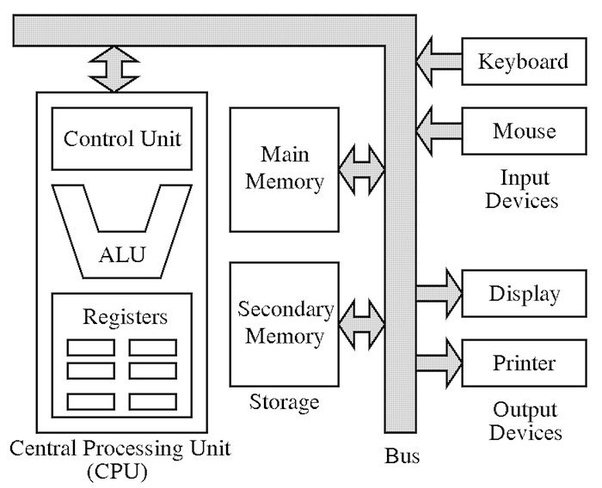
\includegraphics[scale=0.55]{0_von_neumann.png}
	\caption{Architettura di Von Neumann.}
	\label{fig:von_neumann}
\end{figure}

\par %\bigskip
\noindent
La struttura così costituita è composta da tre componenti fondamentali a cui vanno ad aggiungersi le periferiche collegate tramite un modulo di input - output. Tali componenti sono:
\begin{itemize}
	\item Il sistema di memoria, dove risiedono le istruzioni ed i dati necessari all'esecuzione del programma. La memoria può essere costituita da diversi livelli gerarchici. In linea generale si può considerare il \textquotedblleft sistema di memoria" come una memoria principale di tipo RAM nella quale, a runtime, siano già precaricate le istruzioni ed i dati relativi al programma in esecuzione. La memoria può essere vista come un insieme di registri indirizzabili singolarmente e di tipo general purpose, aventi ossia la possibilità di mantenere dati ed istruzioni.
	\item Il sistema di calcolo centralizzato (CPU) che si occupa delle fasi di esecuzione delle istruzioni caricate nella memoria, ossia di eseguire le fasi di FETCH, DECODE, EXECUTE, WRITE BACK per ogni singola istruzione. Al suo interno contiene il sistema di calcolo aritmetico-logico (ALU), l'unità di controllo ed un banco di registri ad alta velocità nel quale i dati vengono salvati mano a mano che viene eseguito il processamento di un'istruzione.
	\item il BUS, che interconnette con la CPU la memoria ed i dispositivi di ingresso - uscita facenti parte del sistema. \'E un bus unico per dati, istruzioni e comandi di controllo, pertanto costituisce un limite prestazionale di tale architettura di calcolo.
\end{itemize}
Come detto su tale architettura è possibile definire un insieme delle istruzioni elementari eseguibili, denominato \textit{instruction-set}. All'interno dell'instruction-set sono disponibili le istruzioni, i registri, le modalità di indirizzamento, l'architettura della memoria, la gestione degli interrupt e delle eccezioni, ed eventualmente l'indirizzamento per i dispositivi di I/O esterni.\\
La combinazione degli elementi presenti all'interno dell'instruction-set in maniera non univoca e più o meno efficiente, permette l'implementazione di un algoritmo fisicamente eseguibile sull'architettura hardware adottata.
L'instruction-set corrisponde dunque a un'interfaccia tra software ed hardware che permette al progettista dell'algoritmo di operare in maniera più semplice sui dispositivi e i segnali interni al sistema digitale col fine dell'implementazione dell'algoritmo stesso.\\
La progettazione dell'instruction-set dipende dall'architettura adottata nel progetto dell'esecutore, differenziando tra sistemi di tipo \textquotedblleft general purpose" come i microprocessori o \textquotedblleft special purpose" come ad esempio i microcontrollori.
A titolo di esempio di un noto set di istruzioni si riporta di seguito quello relativo al microprocessore Intel 4004, il primo microprocessore integrato a 4 bit rilasciato da Intel nel 1971.
\newpage \null \vfill
\begin{figure}[H]
	\centering
	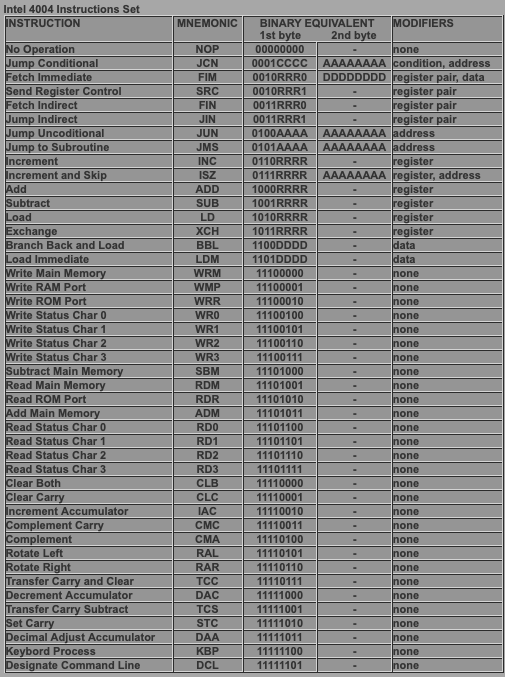
\includegraphics[scale=0.75]{0_4004_instruction_set.png}
	\caption{Il set di istruzioni relativo al microprocessore Intel 4004}
	\label{fig:4004_instruction_set}
\end{figure}
\newpage

\subsection*{Esecuzione delle istruzioni}
\addcontentsline{toc}{subsection}{Esecuzione delle istruzioni}
Sulla base dell'architettura di Von Neumann esposta, a partire dall'instruction-set precedentemente definito, è possibile implementare un algoritmo specifico combinando le istruzioni con i dati che realizzano la funzione desiderata. In prima approssimazione si può pensare che dati e programmi relativi a tale algoritmo siano presenti all'interno della memoria del sistema in maniera sequenziale e sotto forma di linguaggio macchina.\\
Prendendo ad esempio un programma in grado di realizzare la somma tra due valori binari caricati all'interno di altrettanti registri (denominati DR1 e DR2) e il salvataggio del risultato su di un terzo registro (denominato RIS), si avrà il seguente codice assembler:
\begin{lstlisting}[frame=single] 
MV DR1, OP1					 % copia il valore di DR1 in OP1
MV DR2, OP2				 	% salva il valore di DR2 in OP2
SUM				% somma OP1 e OP2 (risultato in ACC)
MV ACC, RIS				% salva il valore di ACC in RIS
\end{lstlisting}
in cui le etichette dei registri corrispondono ad un identificativo hardware (indirizzo) anch'esso definito all'interno dell'instruction-set.
In memoria RAM saranno presenti quindi le istruzioni ed i dati derivanti da tale esempio di programma in maniera sequenziale e come riportato nella figura seguente.
\begin{table}[H]
	\centering
	\begin{tabular}{l|p{2cm}|}
		\cline{2-2} \multicolumn{0}{c|}{0x00} & \makebox[2cm][c]{\textbf{MV}}\\
		\cline{2-2} \multicolumn{0}{c|}{0x01} & \makebox[2cm][c]{DR1}\\
		\cline{2-2} \multicolumn{0}{c|}{0x02} & \makebox[2cm][c]{OP1}\\
		\cline{2-2} \multicolumn{0}{c|}{0x03} & \makebox[2cm][c]{\textbf{MV}}\\
		\cline{2-2} \multicolumn{0}{c|}{0x04} & \makebox[2cm][c]{DR2}\\
		\cline{2-2} \multicolumn{0}{c|}{0x05} & \makebox[2cm][c]{OP2}\\
		\cline{2-2} \multicolumn{0}{c|}{0x06} & \makebox[2cm][c]{\textbf{SUM}}\\
		\cline{2-2} \multicolumn{0}{c|}{0x07} & \makebox[2cm][c]{\textbf{MV}}\\
		\cline{2-2} \multicolumn{0}{c|}{0x07} & \makebox[2cm][c]{ACC}\\
		\cline{2-2} \multicolumn{0}{c|}{0x09} & \makebox[2cm][c]{RIS}\\
		\cline{2-2} \multicolumn{0}{c|}{0x0A} & \makebox[2cm][c]{\textbf{END}}\\
		\cline{2-2} \multicolumn{0}{c|}{} & \makebox[2cm][c]{...}\\
		\multicolumn{0}{c|}{} & \makebox[2cm][c]{...}\\ \cline{2-2}
		\multicolumn{0}{c|}{0xFF} & \makebox[2cm][c]{...}\\ \cline{2-2}
	\end{tabular}
	%\caption*{Organizzazione della memoria relativa al programma d'esempio }
\end{table}
\noindent
L'esecuzione di un'istruzione avviene col ciclo di \textit{fetch-execute}, mantenuto da parte dell'unità di processamento centrale CPU.
Al suo interno sono infatti presenti tutti i sistemi relativi alla sequenziazione delle operazioni (unità di controllo CU), al calcolo aritmetico nonché registri di appoggio dedicati al salvataggio di dati temporanei ed inidirzzamento della memoria.
\begin{figure}[H]
	\centering
	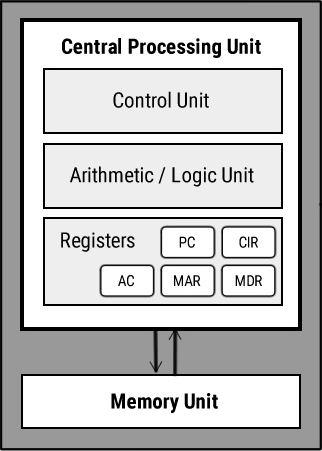
\includegraphics[scale=0.5]{0_vn_cpu.png}
	\caption{La CPU all'interno di un sistema alla Von Neumann}
	\label{fig:vn_cpu}
\end{figure}
\noindent
Nel caso pratico dell'esempio precedentemente riportato, all'avvio dell'esecuzione del programma la CPU darà il comando di \textit{fetch} dell'istruzione presente nella locazione di memoria avente indirizzo 0x00.\\
Al riconoscimento dell'istruzione (\textit{fase di decode}) il sistema diviene al corrente del fatto che ai successivi due prelievi dalla memoria corrisponderanno gli operandi dell'istruzione precedentemente caricata.\\
La fase di \textit{execute} inizia con il prelievo dei dati dagli indirizzi 0x01 e 0x02. Avendo quindi caricato i dati relativi alla prima MOVE il sistema esegue l'istruzione che ha come risultato il salvataggio nel registro denominato OP1 del valore contenuto nel registro denominato DR1.\\
A seguire il sistema esegue a seconda istruzione (prelevata all'indirizzo 0x03 ripetendo quanto detto con la prima MOVE) che termina col salvataggio del dato presente in DR2 sul registro OP2.\\
Al prelievo dell'istruzione all'indirizzo 0x06, corrispondente alla SUM, il sistema esegue la somma dei valori caricati sui registri OP1 ed OP2, precedentemente aggiornati ai valori desiderati. La somma termina col salvataggio del risultato sul registro accumulatore interno (denominato ACC). Infine, con l'istruzione 0x07 si esegue una ulteriore MOVE del dato salvato in ACC sul registro denominato RIS.
Il programma termina con l'esecuzione dell'istruzione all'indirizzo 0x0A e denominata END, che comunica alla macchina il termine delle operazioni del programma.
\par \bigskip
\noindent
L'esecuzione delle istruzioni in questo modello architetturale di memoria prevede il fatto che i dati ed i programmi siano caricati in maniera sequenziale nelle locazioni di memoria. L'indirizzamento della memoria è affidato ad un particolare registro denominato \textquotedblleft Program-Counter", abbreviato con l'identificativo PC. Il valore mantenuto all'interno del PC costituisce quindi l'indirizzo della istruzione in esecuzione o del dato relativo all'istruzione che lo necessita. All'avvenuto prelievo dell'istruzione o del dato corrente (o comunque prima del prelievo della successiva) il PC viene incrementato di 1 puntando di fatto alla successiva locazione di memoria che conterrà un dato o una nuova istruzione.\\
Inoltre poiché si è supposto che l'avvio dell'esecuzione del programma parta dal fetch dell'istruzione all'indirizzo 0x00, allora questa locazione deve necessariamente contenere la prima istruzione che costituisce l'inizio dell'algoritmo.
\par \bigskip \noindent
Quanto detto costituisce un limite prestazionale all'impiego dell'architettura di Von Neumann in quanto la presenza di un unico bus per dati ed istruzioni (e segnali di controllo) limita fortemente le prestazioni di throughput dei dati da parte del sistema. Unitamente a questo limite prestazionale derivante dall'architettura stessa, la gestione della memoria come descritta, ossia contenente i dati relativi alle istruzioni nelle locazioni di memoria strettamente successive alle istruzioni stesse, non permette la realizzazione di tecniche di parallelizzazione volte all'incremento delle prestazioni del sistema.\\ Per tale motivo nel seguente paragrafo verrà descritto un sistema di gestione della memoria più efficiente e compatibile con le tecniche di parallelizzazione.

\subsection*{Von Neumann migliorato}
\addcontentsline{toc}{subsection}{Von Neumann migliorato}
Una soluzione al problema descritto nelle ultime righe del precedente paragrafo prevede la modifica della gestione della memoria nel salvataggio di dati e istruzioni. Questa può essere concettualmente divisa in due aree, una dove vengono salvate in sequenza le istruzioni da eseguire, l'altra che contiene i dati relativi a tali istruzioni, come schematizzato nella figura successiva.
\begin{figure}[H]
	\centering
	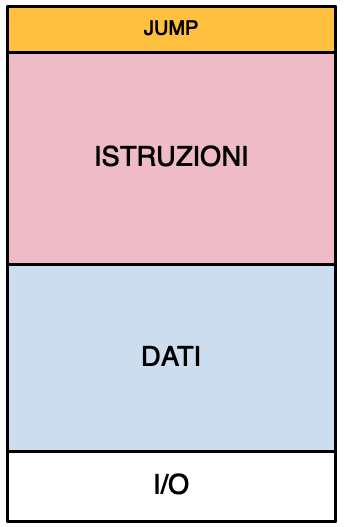
\includegraphics[scale=0.4]{0_memoria_separata.png}
	\caption{Gesione della memoria in un'architettura di Von Neumann migliorata}
	\label{fig:vn_mem}
\end{figure}
\noindent
In tale architettura la gestione della memoria prevede, oltre al classico puntatore all'istruzione denominato program-counter, un puntatore al dato denominato data-counter, abbreviato DC. Tale puntatore contiene l'indirizzo da fornire alla memoria per il prelievo del dato relativo alla istruzione che lo necessita. In questo modo si riescono a garantire due importanti prerogative:
\begin{itemize}
	\item Nel caso in cui non si debba effettuare un salto l'indirizzo relativo alla prossima istruzione è sempre dato dall'indirizzo corrente di PC sommato ad 1.
	\item Nel caso in cui si debba effettuare un salto il valore che punta alla prossima istruzione può già essere puntato da DC e non deve essere ricavato eseguendo un ulteriore aggiornamento di PC per il prelievo di tale dato. In questo modo (nel caso di chiamata a subroutine) il valore di PC può essere salvato come indirizzo di ritorno prima di aggiornare il PC all'indirizzo prelevato dalla memoria e al quale eseguire il salto.
\end{itemize}
L'indirizzamento della memoria si ottiene supponendo delle dimensioni fisse per le aree riservati a istruzioni e dati.\\
Una qualsiasi istruzione presente nell'area dedicata è indirizzabile tramite due coordinate. Una prima fissa, denominata \textit{base istruzione} ed una seconda che indica \textit{l'offset} rispetto a tale base. L'indirizzamento dunque avviene per mezzo del calcolo della seguente somma:
\begin{equation} %\notag
	ADDR_{P} = P_0 + \Delta P
\end{equation} 
Analogamente, in riferimento al calcolo della posizione di un dato si avrà:
\begin{equation}
	ADDR_{D} = D_0 + \Delta D
\end{equation}

\section*{Metodi di indirizzamento}
\label{metodi_di_indirizzamento}
\addcontentsline{toc}{section}{Metodi di indirizzamento}
In base a quanto detto fino ad ora si può procedere alla definizione dell'argomento di questa tesina. Scopo del problema è la progettazione di una UC per un'architettura di Von Neumann curando l'implementazione di parte del set di istruzioni relativo all'indirizzamento della memoria RAM interna, in cui sia prevista la gestione migliorata della memoria precedentemente discussa.\\
In particolare è richiesta l'implementazione delle seguenti istruzioni:
\begin{itemize}
	\item \textbf{RD ADDR}: Esegue una READ della memoria all'indirizzo fornito attraverso il dato ADDR. Il valore letto è salvato su di un registro interno. Per garantire l'indirizzamento di tutto lo spazio di memoria l'operando ADDR è a 2N bit.
	\item \textbf{WR DATA, ADDR}: Esegue la scrittura del valore identificato con DATA nella locuzione di memoria RAM relativa all'indirizzo ADDR. È un'istruzione dal formato \textquotedblleft un'istruzione e due dati".
	Le dimensioni degli operandi: DATA N bit, ADDR 2N bit.
	\item \textbf{JMP ADDR}: Esegue una JUMP incondizionale all'indirizzo presente nel dato ADDR. Tale istruzione realizza un \textquotedblleft \textit{salto immediato}". Il formato dell'istruzione è del tipo \textquotedblleft una istruzione e un dato" ed è a 2N bit.
	\item \textbf{JMP OFFS}: Esegue una JUMP incondizionale all'indirizzo dato dal valore corrente di PC sommato al dato in ingresso denominato OFFS. Costituisce un'istruzione denominata \textquotedblleft \textit{salto diretto}" e prende in ingresso un unico dato. Loperando OFFS ha dimensioni pari a N bit.
	\item \textbf{JMP BASE, OFFS}: Esegue una JUMP incondizionale all'indirizzo calcolato tramite somma dei due dati in ingresso BASE e OFFS. Costituisce un tipo di salto denominato \textquotedblleft \textit{salto indiretto}" e possiede un formato del tipo \textquotedblleft una istruzione e due dati". BASE ed OFFS sono a N bit.
\end{itemize}
Inoltre, dotando la CPU di un insieme di registri interni di tipo \textquotedblleft general-purpose" in appoggio al sistema di calcolo, si implementerà la seguente istruzione:
\begin{itemize}
	\item \textbf{MV REG1, REG2}: Esegue la copia del dato contenuto nel registro avente etichetta REG1 sul registro avente etichetta REG2. Tale istruzione si applica sui registri interni alla CPU.
\end{itemize}

\section*{Istanziazione zero}
\addcontentsline{toc}{section}{Istanziazione zero}
Dunque, in base a quanto esposto precedentemente, si parte con un sistema alla Von Neumann basilare come di seguito nuovamente riportato. All'avvio delle operazioni si suppone che la memoria RAM sia già precaricata con le istruzioni ed i dati nelle aree di memoria dedicate.
\begin{figure}[H]
	\centering
	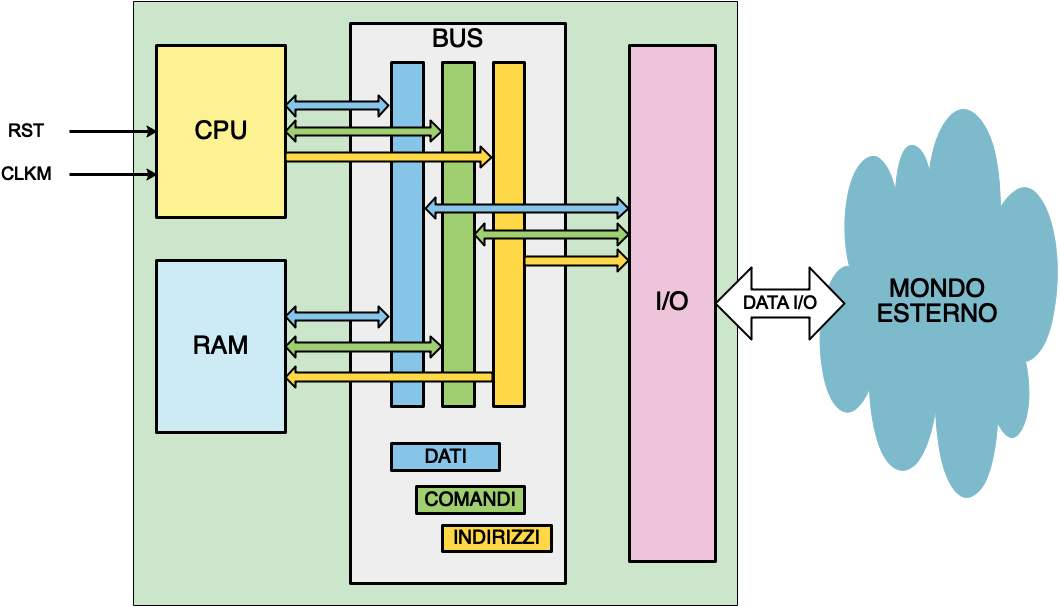
\includegraphics[scale=0.30]{0_ist_zero.png}
	\caption{Struttura interna del sistema in esame}
	\label{fig:ist_0}
\end{figure}
\noindent
Le comunicazioni con l'esterno avvengono per mezzo del bus di I/O ad N bit. Si partirà nello svolgimento del problema tipo \textquotedblleft carta e penna" con un valore per le dimensioni del bus dati pari a $N = 4$. La dimensione del bus indirizzi si sceglie pari a $M=2\cdot N$ bit che definisce uno spazio di indirizzamento della memoria pari a $2^{8} = 256$ parole a N bit. In seguito, su ambiente di sviluppo ISE, si modificherà la dimensione del bus dati (e di conseguenza quella del bus indirizzi) per un valore di N = 8 bit. Dunque i segnali presenti a questo livello di definizione del problema sono i seguenti:
\begin{itemize}
	\item \textbf{OPERANDI E RISULTATO:}
	\begin{itemize}
		\item \textbf{DATA\_IO} (N bit): bus di input-output di collegamento con l'esterno.
	\end{itemize}

	\item \textbf{CLOCK MACCHINA:}
	\begin{itemize}
		\item \textbf{CLKM}: clock macchina per evoluzione sincrona.
	\end{itemize}

	\item \textbf{RESET:}
	\begin{itemize}
		\item \textbf{RST}: \{0: funzionamento normale; 1: reset attivo $\rightarrow$ il sistema riavvia l'esecuzione dalla prima istruzione\}.
	\end{itemize}
\end{itemize}
